To start we designed a small pilot study to validate the classification and clustering methodology against the scale and complexity of data collected on a open public area such as a retail high street.
We also aim to find the algorithm which is best suited for classification of signal strengths to filter out the background noise.
The data was collected at Oxford Street, London on 20 December 2017 from 12:30 to 13:00 hrs, where Wi-Fi probe requests were collected using the sensor described in Chapter \ref{methodology} and pedestrian footfall was manually recorded using the Android app \citep{bala2018clicker}.
Being located at one of the busiest retail locations in the United Kingdom, the Wi-Fi sensor captured approximately 60,000 probe requests during the half hour period, and 3,722 people were recorded manually walking on the sidewalk during that time.

As a first step we just aggregated the probe requests by their MAC address for every minute to generate a minute by minute count of the number of people around the sensor assuming each MAC address corresponds to a mobile device and hence a pedestrian.
We then compare this preliminary `footfall' count to the actual number of pedestrian recorded manually to check for the robustness. We use Mean Absolute Percentage Error (MAPE) measure of robustness of the count since it provides a simple and quick measurement while the street conditions ensure that there are no intervals without any footfall.
We find that the MAPE in the raw counts compared to the ground truth is around 425\%.
This suggests the presence of large amount of noise in the data which might be generated due to sources of uncertainties discussed in Chapter \ref{methodology} thus demonstrating the need for filtering the data.

We then classified the probe requests as ones with "high signal strength" and "low signal strength" using various classification algorithm such as k-means, quantile, hierarchical clusters, fisher and jenks.
We found that while hierarchical clustering and jenks were resource intensive, k-means gave quickest results with the lowest MAPE closely followed by quantile.
The cut-off point or threshold for the collected data with which we could classify them as high and low was -71 dBm.
We then removed all the probe requests which reported `low signal strength' and repeated the same aggregation process as before to produce footfall count. 
This process resulted in a footfall count with a net MAPE of 30\%.
Though the results are encouraging we are still not completely confident that our filtering process is indeed removing noise or has any correlation the configuration of sensor or position of the mobile devices.
These need to be addressed with a larger survey with multiple location of varying orientations.

\begin{figure}
	\centering
	\subfigure[Clustering probe requests based on increasing sequence numbers present in them.]{
		\resizebox*{0.45\linewidth}{!}{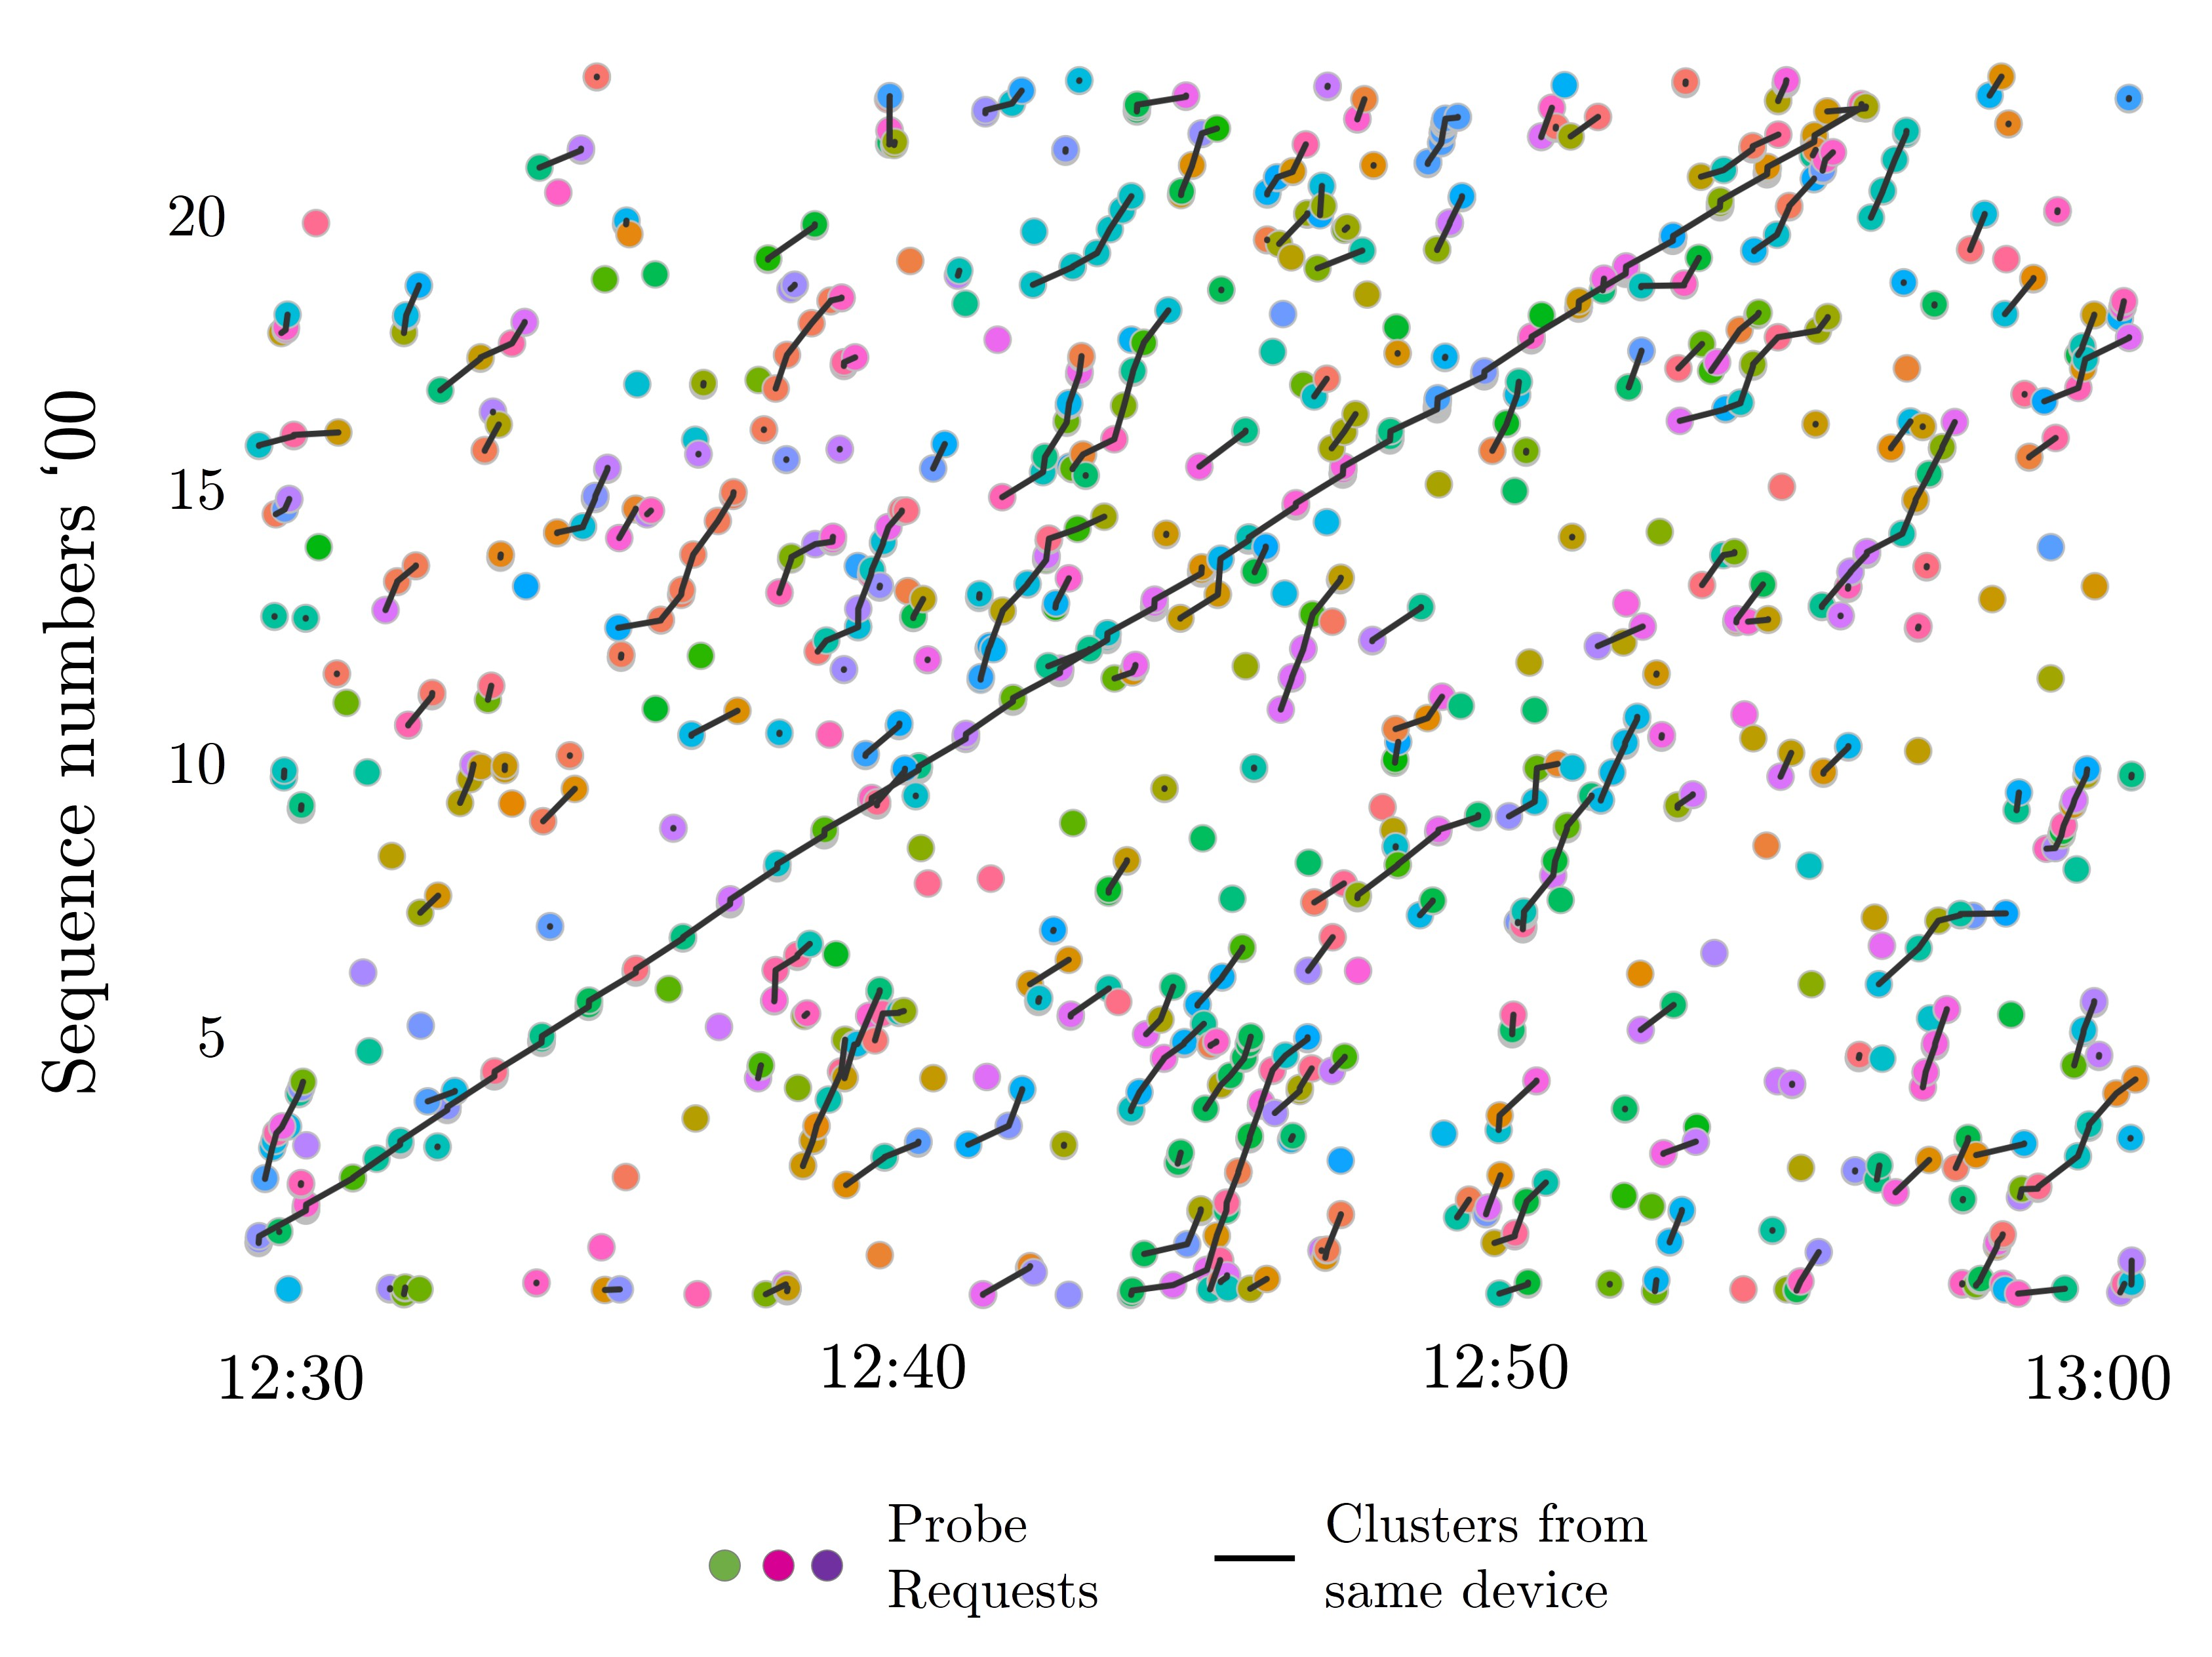
\includegraphics{images/pilot_clustering.jpeg}}}\hspace{20pt}
	\subfigure[Comparison of sensor based counts with the ground truth.]{
	\resizebox*{0.45\linewidth}{!}{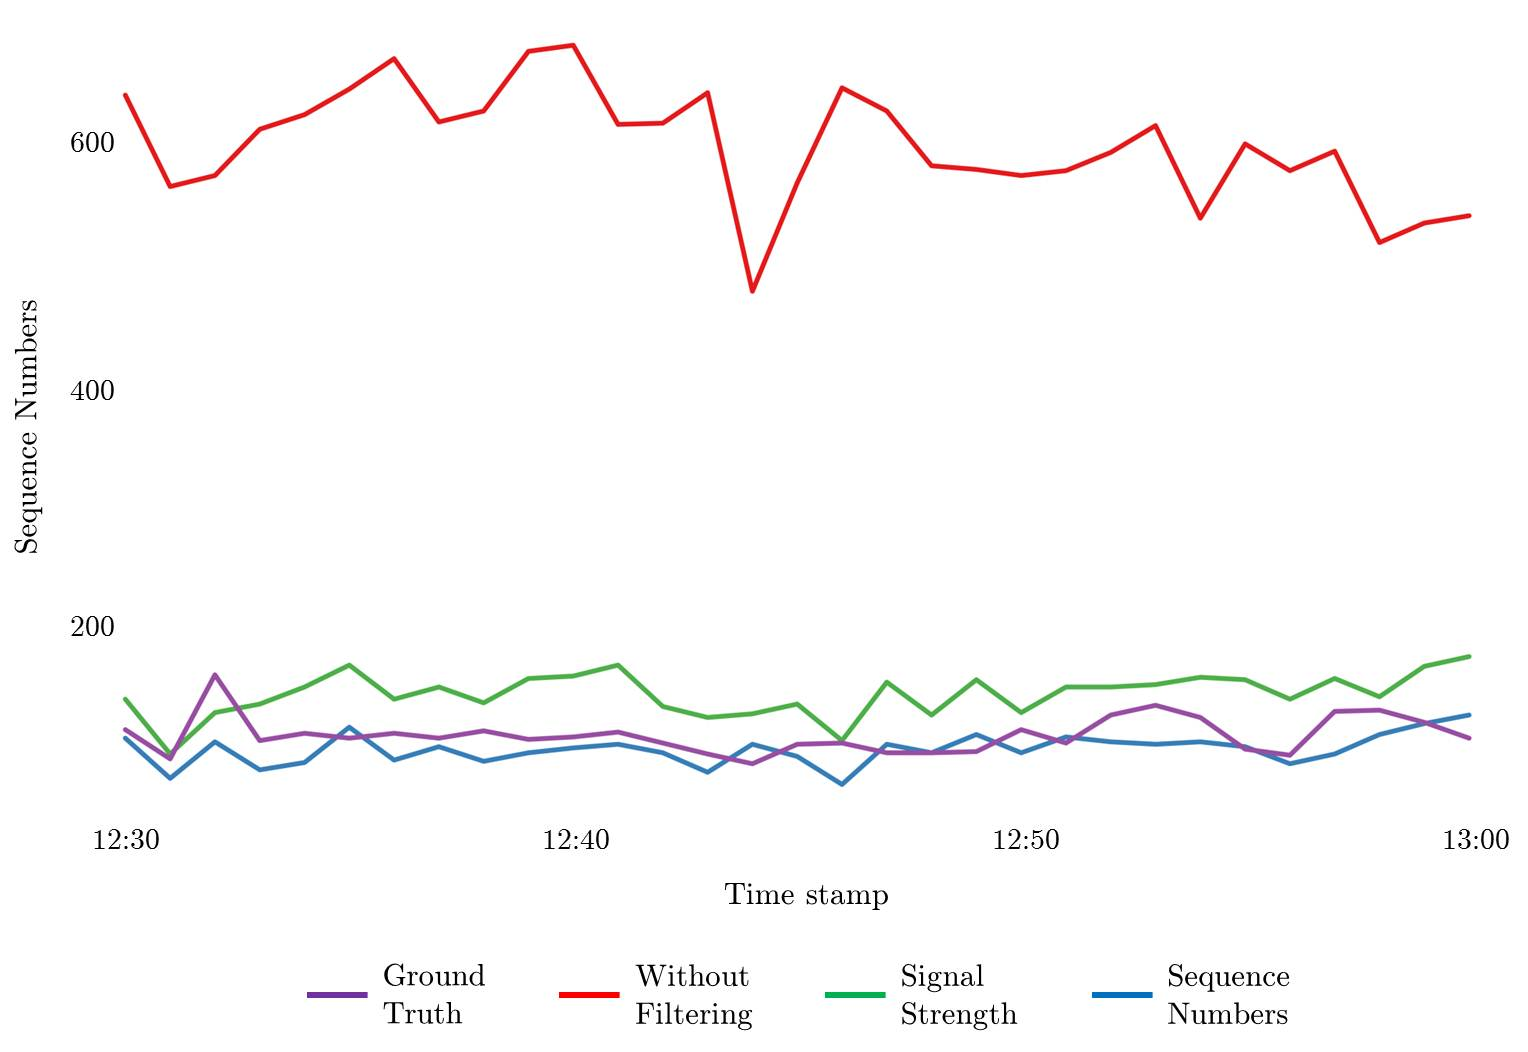
\includegraphics{images/pilot_comparison.jpeg}}}
	\caption{The results of the pilot study demonstrating the validity of the methodology.} \label{pilot_results}
\end{figure}


The next challenge was to identify probe requests which are generated by the same device irrespective of MAC randomisation process.
We use the algorithm defined in Chapter \ref{methodology} and assign a unique identifier or signature to each probe request independent of the MAC address. 
Since there is neither prior research nor documentation on a universal behaviour of phones in randomising their MAC addresses, we use the stationary device - the one used for manual counting as a reference and find out the suitable time threshold, $\alpha$ and threshold for sequence numbers, $\beta$ to be 16s and 60 respectively via trial and error.
This process is done on top the filtering done based on signal strength and only for the probe requests with randomised MAC addresses.
Figure \ref{pilot_results} shows the results of this clustering process on a small set of randomised probe requests.
The probe request with different randomised MAC address is shown by the colored points and the line joining them shows the ones belonging to the same cluster hence expected to be generated by the same device.
We finally aggregate the probe requests as before but with the device signature rather than just MAC addresses this results in a footfall count with a MAPE of -18\%. 
A comparison of minute by minute counts resulting from different filtering processes along with the ground truth is shown in Figure \ref{pilot_results} showing the promising effectiveness of the methods.

To conclude, from the pilot study we found that both classification and clustering methods we devices work on complex real world data and results in a final pedestrian counts within a MAPE of 20\%. We also found `k-means' and `quantile' are best algorithms for classifying signal strengths and the threshold for time and sequence numbers for the clustering algorithm is around 16 and 60 respectively.
